% Copyright 2021 Edoardo Riggio

% Licensed under the Apache License, Version 2.0 (the "License");
% you may not use this file except in compliance with the License.
% You may obtain a copy of the License at

% 	http://www.apache.org/licenses/LICENSE-2.0

% Unless required by applicable law or agreed to in writing, software
% distributed under the License is distributed on an "AS IS" BASIS,
% WITHOUT WARRANTIES OR CONDITIONS OF ANY KIND, either express or implied.
% See the License for the specific language governing permissions and
% limitations under the License.

\documentclass{article}

\usepackage{hyperref, amsmath, graphicx, amssymb}
\usepackage{fancyvrb, newverbs, xcolor, tikz}
\usepackage[latin1]{inputenc}

\usetikzlibrary{positioning}

\graphicspath{{./assets/}}
\definecolor{cverbbg}{gray}{0.93}

\newenvironment{cverbatim}
 {\SaveVerbatim{cverb}}
 {\endSaveVerbatim
  \flushleft\fboxrule=0pt\fboxsep=.5em
  \colorbox{cverbbg}{\BUseVerbatim{cverb}}%
  \endflushleft
}

\newenvironment{lcverbatim}
 {\SaveVerbatim{cverb}}
 {\endSaveVerbatim
  \flushleft\fboxrule=0pt\fboxsep=.5em
  \colorbox{cverbbg}{%
    \makebox[\dimexpr\linewidth-2\fboxsep][l]{\BUseVerbatim{cverb}}%
  }
  \endflushleft
}

\begin{document}
\begin{titlepage}
    \begin{center}
        \vspace*{1cm}
        
        \Huge
        \textbf{Quantum Computing Cheatsheet}
        
        \vspace{0.5cm}
        \LARGE
        
        \vspace{.5cm}
        
        Edoardo Riggio
   		  \vspace{1.5cm}
       
        \vfill
        
        \today
        
        \vspace{.8cm}
          \Large
          Quantum Computing - S.P. 2022 \\
        Computer Science\\
        Universit\`{a} della Svizzera Italiana, Lugano\\
        
    \end{center}
\end{titlepage}

\tableofcontents

\newpage

\section{What is Quantum Informatics}
\subsection{Information and Physics}
Experience, observation, and physical discourse are in the form of information. "It from Bit" -- John Wheeler \\ \\
Information representation, processing, and transmission are physical processes. "Information is physical" -- Rolf Landauer \\ \\
The representation of a bit must be physical. Moreover, digitalization comes very naturally with \textbf{quantization}. In classical physics, digitalization has to be enforced somehow (e.g., switched).

\subsection{Second Law of Thermodynamics}
The second law of thermodynamics states that, in a closed system, entropy does not increase. \\ \\
\textbf{Entropy} can be defined as a measure of disorder. Given $n$ binary memory cells containing random bits, if we erase all of the bits -- i.e., set them to 0 -- then the entropy in the set of memory cells drops.

\subsection{The Stern/Gerlach Experiment}
This experiment was proposed in 1921 by Otto Stern and later carried out in 1922 by Walther Gerlach. \\ \\
This is one of the most important experiments to understand the structure and properties of the basic building block of quantum information processing, the \textbf{Qbit}.

\begin{center}
	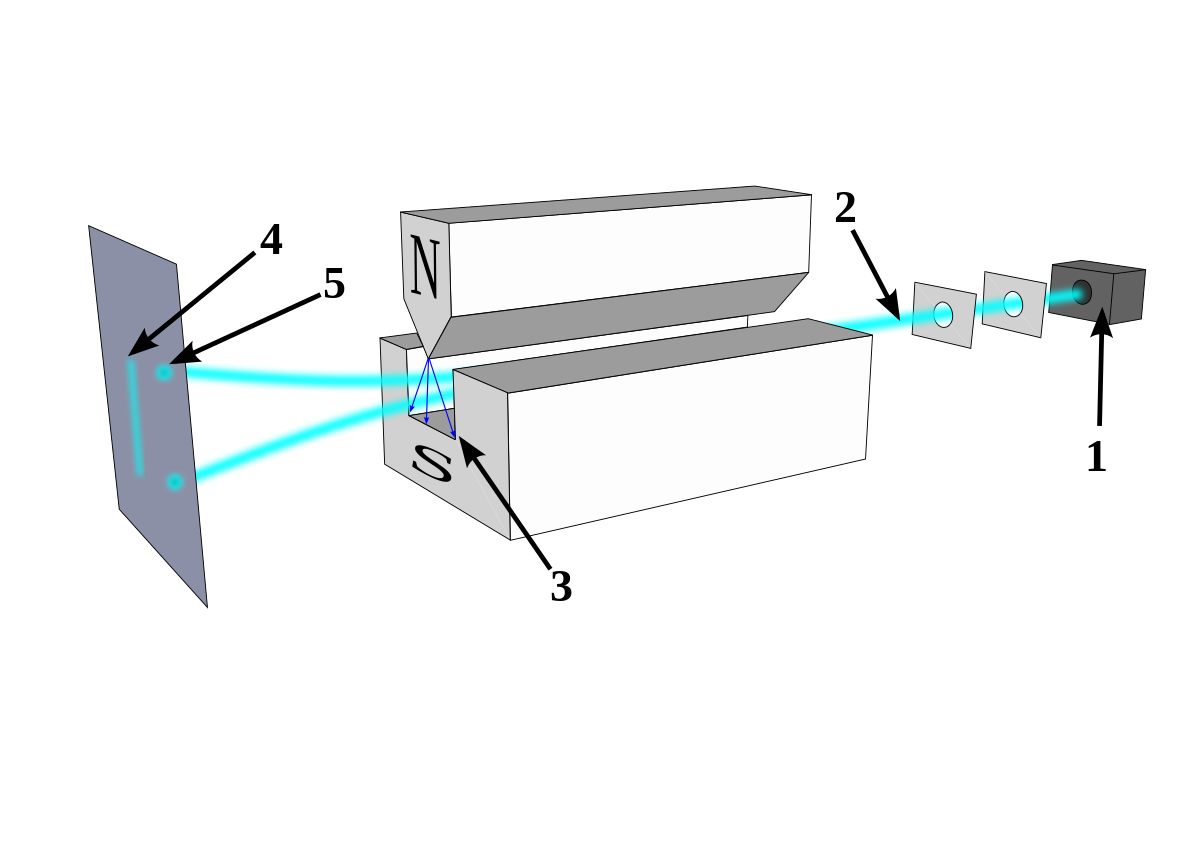
\includegraphics[width=8cm]{assets/stern_gerlach.png}
\end{center}
This experiment consisted of the measurement of the \textbf{magnetic dipole moment} of silver atoms. These silver atoms are sent as a stream (2) coming from an oven (1). Each atom is deflected from the path through an inhomogeneous magnetic field (3), and each atom is deflected from the path (5). This deflection is proportional to its dipole in the direction of the magnets. \\ \\
This experiment revealed no detection in the middle of the screen (4) but rather two sharp peaks at equal distances from the center (5). The quantity measured by the experiment is known in quantum mechanics as \textbf{spin}. \\ \\
In the case of a single measurement, for example, in the $z$-direction, it will result in two identical rays.

\begin{center}
	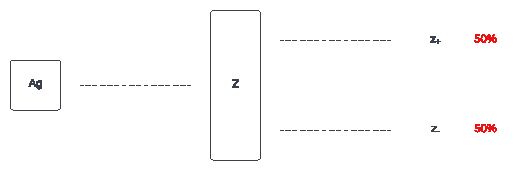
\includegraphics[width=10cm]{assets/one_z_measurement.pdf}
\end{center}
If the exact measurement is repeated for only one of the rays -- say $z_+$, then all the atoms are deflected again in the $+$ direction.

\begin{center}
	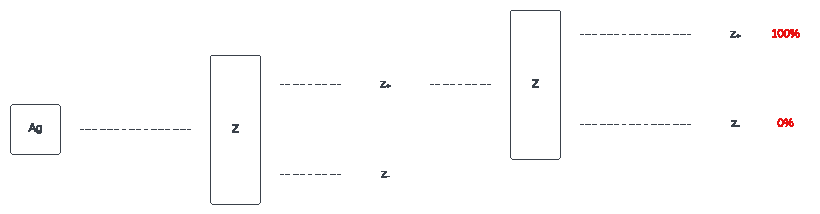
\includegraphics[width=11.5cm]{assets/two_z_measurements.pdf}
\end{center}
Finally, if the magnet is rotated and a $x$-direction measurement of the $z_+$ ray is made, another $z$-direction measurement, a 50-50 distribution. This puts the stability and the independence of the properties in question.

\begin{center}
	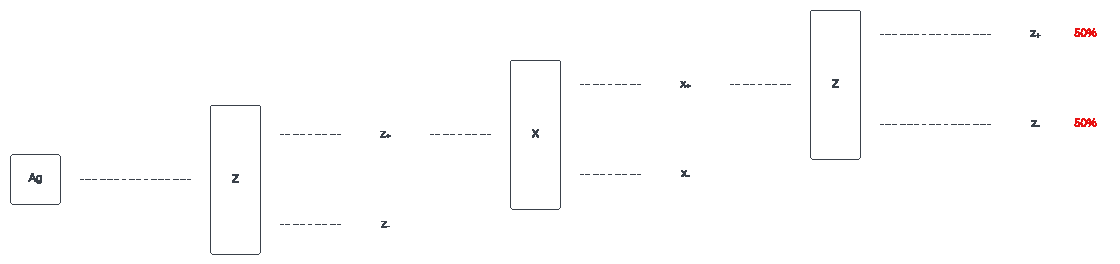
\includegraphics[width=12cm]{assets/z_x_z_measurements.pdf}
\end{center}

\subsection{Superposition}
Quantum superposition is a fundamental principle of quantum mechanics. It states that any two -- or more -- quantum states can be added together, and the result will be another valid quantum state. \\ \\
The question of whether a silver atom is in the state $| z_- \rangle$ or in the state $| z_+ \rangle$ are complementary to one another. They can be regarded as two answers to the same question -- i.e., the $Z$ measurement. \\ \\
If after performing an $X$ measurement, we want to know whether the silver atom is in a state $| x_+ \rangle$ or $| x_- \rangle$. Both are qual superpositions
\[ |x_+\rangle = \frac{1}{\sqrt{2}}|z_+\rangle + \frac{1}{\sqrt{2}}|z_-\rangle \]
\[ |x_-\rangle = \frac{1}{\sqrt{2}}|z_+\rangle - \frac{1}{\sqrt{2}}|z_-\rangle \]
No matter if we obtain one measurement or the other in the $Z$ measurement, the $X$-measurement either $| x_+ \rangle$ or $| x_- \rangle$ with equal probability. This is also known as a \textbf{quantum jump}.

\begin{center}
	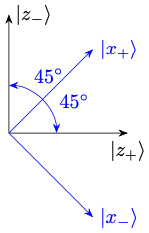
\includegraphics[width=2cm]{quantum_jump.png}
\end{center}

\subsection{Quantum Key Distribution}
We have seen that we can measure with certainty the same value in two consecutive measurements with the same basis. In other words, the interactions of a system with its environment become traceable. This traceability enables us to detect an eavesdropper in a \textbf{quantum cryptographic key agreement protocol}. \\ \\
The distribution of the key starts with \textit{Alice} using random measurements to encrypt the data. The encrypted photons are then sent to \textit{Bob}, which also uses random measurements to try and decrypt the data. After this process has terminated, \textit{Alice} sends the measurement basis she used to \textit{Bob} on a public channel. \textit{Bob} now takes the measurement basis and confronts it with his basis. The equal measurements are used as the \textbf{key}. \\ \\
If an eavesdropper, say \textit{Eve}, tries to intercept the message, she will need to guess the measurements for each photon. If the measurement is wrong, the system is disturbed. This means that \textit{Eve} has a probability of $1/4$ to be wrong in each stage. Thus, there is an almost 100\% probability of whether there was an eavesdropper.

\section{Glossary}
\subsection{Magnetic Dipole Moment}
The magnetic dipole moment is a vector that represents the strength and orientation of a magnet or other object that produces a magnetic field (e.g., an electron).

\end{document}

































